\defcitealias{Tarango-Yong:2018a}{Paper~I}
\newcommand\PaperI{\citetalias{Tarango-Yong:2018a}}

\section{Introduction}
\label{sec:introduction}
\newcommand\hii{\ion{H}{ii}}

Curved emission arcs around stars \citep[e.g.,][]{Gull:1979a} are
often interpreted as \textit{bow shocks}, due to a supersonic
hydrodynamic interaction between the star's wind and an external
stream. This stream may be due to the star's own motion or to an
independent flow, such as an \hii{} region in the champagne phase
\citep{Tenorio-Tagle:1979a}, or another star's wind
\citep{Canto:1996}. However, an alternative interpretation in some
cases may be a radiation-pressure driven bow wave, as first proposed
by \citet[\S\textsc{vi}]{van-Buren:1988a}.  In this scenario, photons
emitted by the star are absorbed by dust grains in the incoming
stream, with the resultant momentum transfer being sufficient to
decelerate and deflect the grains within a certain distance from the
star, forming a dust-free, bow-shaped cavity with an enhanced dust
density at its edge.  Two regimes are possible, depending on the
strength of coupling between the gas (or plasma) and the dust.  In the
strong-coupling regime, gas--grain drag decelerates the gas along with
the dust, forming a shocked gas shell in a similar fashion to the
wind-driven bow shock case.  In the weak-coupling regime, the gas
stream is relatively unaffected and the dust temporarily decouples to
form a dust-only shell.  This second case has recently been studied in
detail in the context of the interaction of late O-type stars (which
have only weak stellar winds) with dusty photoevaporation flows inside
\hii{} regions \citep{Ochsendorf:2014a, Ochsendorf:2014b,
  Ochsendorf:2015a}.  We follow the nomenclature proposed by
\citet{Ochsendorf:2014b}, in which \textit{dust wave} refers to the
weak coupling case and \textit{bow wave} to the strong coupling case.
More complex, hybrid scenarios are also possible, such as that studied
by \citet{van-Marle:2011a}, where a hydrodynamic bow shock forms, but
the larger dust grains that accompany the stellar wind pass right
through the shocked gas shell, and form their own dust wave at a
larger radius.

\begin{figure}
  \centering
  \framebox{
    \parbox[m][4cm]{0.8\linewidth}
    {\centerline{\textbf{\dotfill TODO\dotfill}}}}
  \caption{Bow shocks, bow waves, and dust waves}
  \label{fig:3-types-bow}
\end{figure}

In \citet[][hereafter \PaperI{}]{Tarango-Yong:2018a}, we proposed a
new two-dimensional classification scheme for bow shapes: the
projected planitude--alatude, or \(\Pi'\)--\(\Lambda'\), diagram.  Planitude
measures the flatness of the bow's apex, while alatude measures the
openness of the bow's wings.  Both are dimensionless ratios of lengths
that can be estimated from observational images.  We have analyzed the
inclination-dependent tracks on the \(\Pi'\)--\(\Lambda'\) plane for simple
geometric shapes (spheroids, paraboloids, hyperboloids) and for
thin-shell hydrodynamic bow shock models (wilkinoid, cantoids,
ancantoids).  In this paper, we will do the same for simple models of
radiation-driven dust waves (dragoids) and bow waves (trapoids).

The paper is organized as follows.
%
In \S~\ref{sec:shape-dust-wave} we do the same for simple models of a
dusty radiation bow wave (dragoids), including the effects of
gas-grain drag.
%
In \S~\ref{sec:perturbed-bows} we investigate the effects on the
planitude--alatude plane of small-amplitude perturbations to the bow
shape.
%


\section{Different types of bow}
\label{sec:different-types-bow}

\begin{figure*}
  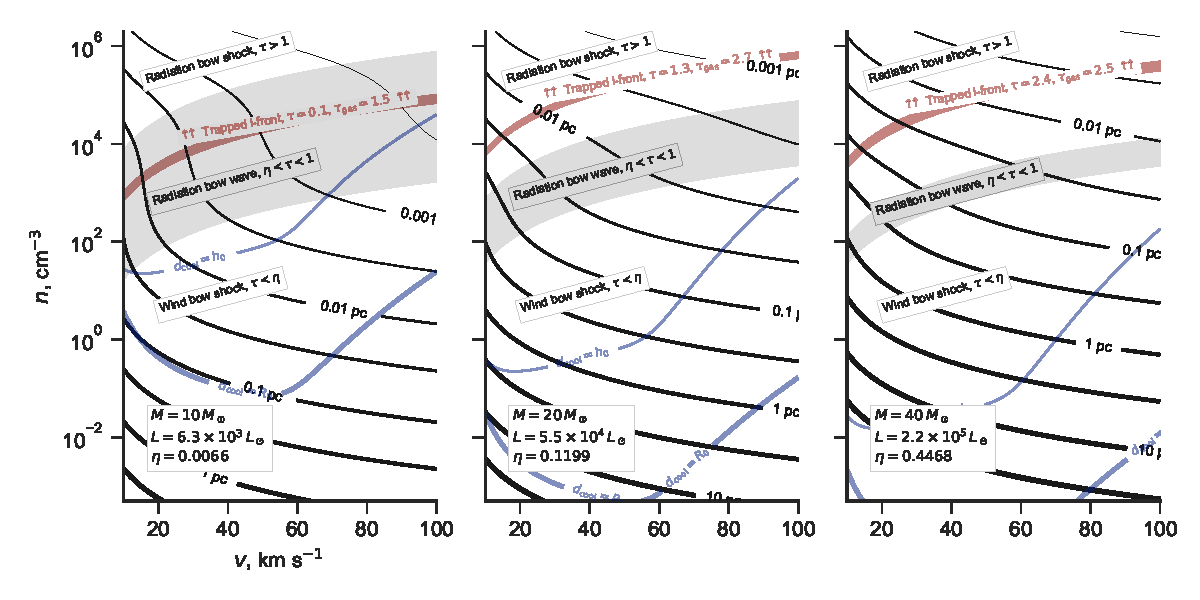
\includegraphics[width=\linewidth]{figs/zones-v-n-plane}
  \caption{Bow regimes of parameter space (\(v, n\)) of the external
    stream for main-sequence OB stars of different masses:
    (a)~\SI{10}{M_\odot}, (b)~\SI{20}{M_\odot}, (c)~\SI{40}{M_\odot}. }
  \label{fig:zones-v-n-plane}
\end{figure*}

We will mainly consider the canonical case of a bow around a star of
bolometric luminosity, \(L\), with a radiatively driven
wind,\footnote{In \S~\ref{sec:case-inside-out} we consider the case of
  an external luminous source.} which is immersed in an external
stream of gas and dust with density, \(\rho\), and velocity, \(v\).  The
size and shape of the bow is determined by a generalized balance of
pressure (or, equivalently, momentum) between internal and external
sources.  We assume that the stream is supersonic and super-alfvenic,
so that the external pressure is dominated by the ram pressure:
\(\rho v^2\). We first consider the case where the dust grains and gas
are perfectly coupled by collisions (although this assumption is
relaxed below in \S~\ref{sec:imperf-coupl-betw}).

The internal pressure is the sum of wind ram pressure and the
effective radiation pressure that acts on the bow shell.  The
radiative momentum loss rate of the star is \(L/c\) and the wind
momentum loss rate can be expressed as
\begin{equation}
  \label{eq:wind-efficiency}
  \dot{M} V = \eta L / c \ , 
\end{equation}
where \(\eta\) is the momentum efficiency of the wind, which is typically
\(< 1\) \citep{Lamers:1999b}. If the optical depth is very large, then
all of the stellar radiative momentum, emitted with rate \(L/c\), is
trapped by the bow shell.  In the single scattering
limit,\footnote{Why multiple scattering is not important.} and
temporarily neglecting the wind, then pressure balance at the bow
apex, a distance \(R_0\) along the symmetry axis from the star is given by
\begin{equation}
  \label{eq:rad-press-balance-thick}
  \frac{L}{4 \pi c R_0^2} = \rho v^2 \ ,
\end{equation}
which gives a fiducial bow shock radius in this optically thick limit
as
\begin{equation}
  \label{eq:Rstar}
  R_* = \left(\frac{L}{4\pi c \rho v^2}\right)^{1/2} \ .
\end{equation}

We now consider the opposite, optically thin limit.  Although dust
grains typically constitute only a small fraction
\(Z\grain \sim 0.01\) of the mass of the external stream, they
nevertheless dominate the broad-band opacity at FUV, optical and IR
wavelengths if they are present.\footnote{%
  At EUV wavelengths (\(\lambda < \SI{912}{\angstrom}\)), gas opacity
  dominates if the hydrogen neutral fraction is larger than
  \(\approx 0.001\), see discussion of ionization front trapping
  below.} %
If the total opacity (gas plus dust) per total mass (gas plus dust) is
\(\kappa\) (with units of \si{cm^2.g^{-1}}), then the radiative
acceleration in the optically thin limit is
\begin{equation}
  \label{eq:rad-accel}
  a_{\text{rad}} = \frac{\kappa L}{4 \pi c R^2} \ , 
\end{equation}
so that an incoming stream with initial velocity, \(v_\infty\), can be
brought to rest by radiation alone\footnote{%
  For simplicity, we here ignore the effects of pressure gradients and
  shocks, which are important as the velocity approaches the sound
  speed, \(\sound\). In \S~XX below, we show that the resultant
  corrections to \(R_0\) are of order \(\sound / v_\infty\).} %
at a distance \(R_0\) where
\begin{equation}
  \label{eq:rad-poten}
  \int_{R_0}^\infty a_{\text{rad}} \, dr = \tfrac12 v^2 \ , 
\end{equation}
yielding
\begin{equation}
  \label{eq:rad:R0}
  R_0 = \frac{\kappa L}{2\pi c v_\infty^2} \ .
\end{equation}
On the other hand, we can also employ a similar argument to the
optically thick case above by approximating the bow shell as a
surface, and balancing stellar radiation pressure against the ram
pressure of the incoming stream.  The important difference when the
shell is not optically thick is that only a fraction \(1 - e^{-\tau}\) of
the radiative momentum is absorbed by the bow, so that equation~\eqref{eq:rad-press-balance-thick} is replaced with 
\begin{equation}
  \label{eq:rad-press-balance-tau}
  \frac{L (1 - e^{-\tau})}{4 \pi c R_0^2} = \rho v^2 \ .
\end{equation}
In the optically thin limit, \(1 - e^{-\tau} \approx \tau\), so these two
descriptions can be seen to agree so long as
\(\tau = 2 \kappa \rho R_0\), which we will assume to be generally valid.

Then, defining a fiducial optical depth, \(\tau_* = \rho \kappa R_*\), and adding
in the stellar wind ram pressure\footnote{%
  We implicitly assume that the interaction of the stellar wind with
  the external stream can always be treated in the continuum limit.
  This will be true if either the collisional mean free path or the
  ion Larmor radius is much smaller than \(R_0\), which is almost
  always the case.} %
from equation~\eqref{eq:wind-efficiency}, we find that the general bow
radius can be written in terms of the fiducial radius as
\(R_0 = x R_*\), where \(x\) is the solution of
\begin{equation}
  \label{eq:rad-full-x}
  x^2 - \bigl(1 - e^{-2 \tau_* x} \bigr) - \eta = 0 \ .
\end{equation}
Since this is a transcendental equation, \(x\) must be found
numerically, but we can write explicit expressions for three limiting
cases:
\begin{equation}
  \label{eq:x-cases}
  x \approx
  \begin{cases}
    \text{if \(\tau_* \gg 1\):} & (1 + \eta)^{1/2} \\
    \text{if \(\tau_*^2 \ll 1\):} & \tau_* + \bigl( \tau_*^2 + \eta \bigr)^{1/2} \approx
    \begin{cases}
      \text{if \(\tau_*^2 \gg \eta\):} & 2 \tau_* \\
      \text{if \(\tau_*^2 \ll \eta\):} & \eta^{1/2} 
    \end{cases}
  \end{cases}
\end{equation}
The first case, \(x \approx (1 + \eta)^{1/2}\), corresponds to a
\textit{radiation bow shock}; the second case,
\(x \approx 2 \tau_* \), corresponds to a \textit{radiation bow wave}; and the
third case, \(x \approx \eta^{1/2}\), corresponds to a \textit{wind bow shock}.
The two bow shock cases are similar in that the external stream is
oblivious to the presence of the star until it suddenly hits the bow
shock shell, differing only in whether it is radiation or wind that is
providing the internal pressure.  In the intermediate bow wave case,
on the other hand, the external stream is gradually decelerated by
absorption of photons as it approaches the bow.\footnote{A shock does
  still form in this case, but shocked material constitutes a small
  fraction of the total column density of the shell, see \S~XX.}

We now consider the application to bow shocks around main sequence OB stars. 

\subsection{Imperfect coupling between gas and dust}
\label{sec:imperf-coupl-betw}

\begin{figure}
  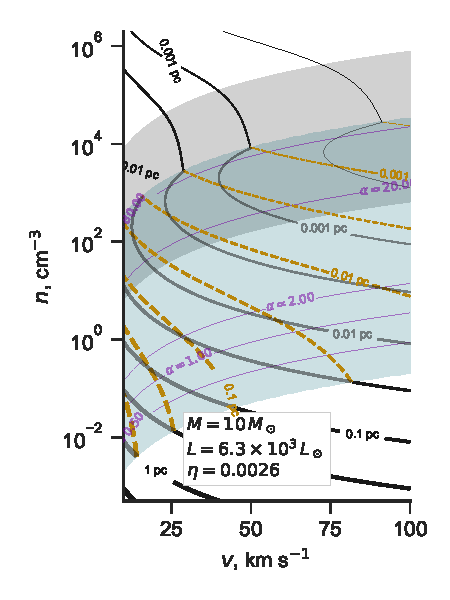
\includegraphics[width=\linewidth]{figs/decouple-v-n-plane}
  \caption{As Fig.~\ref{fig:zones-v-n-plane}(a), but accounting for
    gas-grain decoupling with constant efficiency \(\xi = 0.07\). }
  \label{fig:decouple-v-n-plane}
\end{figure}

\begin{figure}
  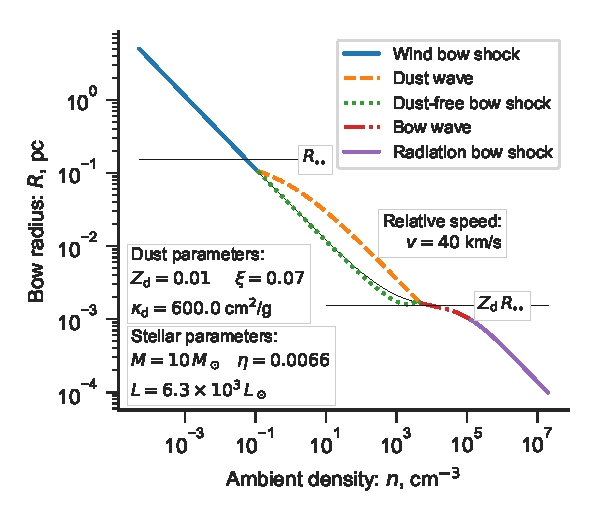
\includegraphics[width=\linewidth]{figs/decouple-v40-versus-n}
  \caption{Vertical cut through Fig.~\ref{fig:decouple-v-n-plane},
    showing bow radius and different regimes for a fixed inflow
    velocity of \SI{40}{km.s^{-1}}.}
  \label{fig:decouple-v40-versus-n}
\end{figure}


\subsection{The case of inside-out bows with external illumination}
\label{sec:case-inside-out}


%%% Local Variables:
%%% mode: latex
%%% TeX-master: "dusty-bow-wave"
%%% End:
